\ifdefined\COMPLETE
\else
\documentclass[12pt]{article}
\usepackage{tikz}
\usetikzlibrary{shapes, calc, arrows, through, intersections, decorations.pathreplacing, patterns}

\begin{document}
\fi

\def\alph{$2+\sqrt{5}$}
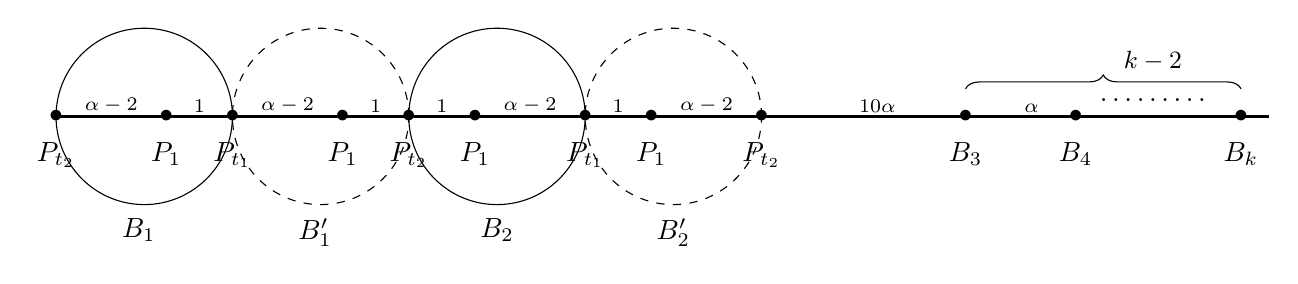
\begin{tikzpicture}[scale=7]

	\coordinate (x) at ($ (-0.20,{sqrt(0)}) $);
	\coordinate (y) at (2.0,0);
	\draw[thick] (x) --(y);

	\node[label=270:$P_{t_2}$] at (-0.20,0) {$\bullet$};
	\node[label={[yshift=-0.2cm]\scriptsize $\alpha-2$}] at (-0.1,0) {};
	\node[label=270:$P_1$] at (0.0,0) {$\bullet$};
	\node[label={[yshift=-0.2cm]\scriptsize $1$}] at (0.06,0) {};
	\node[label=below:{$P_{t_1}$}] at (0.12,0) {$\bullet$};
	\node[label={[yshift=-0.2cm]\scriptsize $\alpha-2$}] at (0.22,0) {};
	\node[label=270:$P_1$] at (0.32,0) {$\bullet$};
	\node[label={[yshift=-0.2cm]\scriptsize $1$}] at (0.38,0) {};
	\node[label=270:$P_{t_2}$] at (0.44,0) {$\bullet$};
	\node[label={[yshift=-0.2cm]\scriptsize $1$}] at (0.5,0) {};
	\node[label=270:$P_1$] at (0.56,0) {$\bullet$};
	\node[label={[yshift=-0.2cm]\scriptsize $\alpha-2$}] at (0.66,0) {};
	\node[label=270:$P_{t_1}$] at (0.76,0) {$\bullet$};
	\node[label={[yshift=-0.2cm]\scriptsize $1$}] at (0.82,0) {};
	\node[label=270:$P_1$] at (0.88,0) {$\bullet$};	
	\node[label={[yshift=-0.2cm]\scriptsize $\alpha-2$}] at (0.98,0) {};
	\node[label=270:$P_{t_2}$] at (1.08,0) {$\bullet$};	
	\node[label={[yshift=-0.2cm]\scriptsize $10\alpha$}] at (1.29,0) {};
	\node[label=270:$B_3$](p3start) at (1.45,0) {$\bullet$};	
	\node[label={[yshift=-0.2cm]\scriptsize $\alpha$}] at (1.57,0) {};
	\node[label=270:$B_4$](B) at (1.65,0) {$\bullet$};	
	\node at (1.79,0.03) {$\ldots\ldots\ldots$};	
	\node[label=270:$B_k$](p3end) at (1.95,0) {$\bullet$};	
	\node(A) at (1.79,0.1) {\small $k-2$};	
	
	\node[label=270:$B_1$] at (-0.05,-0.15) {};	
	\node[label=270:$B_1'$] at (0.27,-0.15) {};	
	\node[label=270:$B_2$] at (0.6,-0.15) {};	
	\node[label=270:$B_2'$] at (0.92,-0.15) {};
	
	\draw (-0.04,0) circle (0.16) ;
	\draw[dashed] (0.28,0) circle (0.16);
	\draw (0.6,0) circle (0.16cm);
	\draw[dashed] (0.92, 0.0) circle (0.16) ;
	\draw[decorate,decoration={brace,amplitude=5pt}]
	(1.45, 0.05) -- (1.95, 0.05);
	%\draw (A) -- (1.74, 0.06);
\end{tikzpicture}


\ifdefined\COMPLETE
\else
\end{document}
\fi
